 
\section*{Aufgabe 1: \emph{1}}


\section*{Aufgabe 2: \emph{Zufallszahlengeneratoren}}

Zufallszahlengenerator mit
\begin{equation}
x_n=(ax_{n-1}+b) \text{ mod } m .
\end{equation}

\begin{itemize}


\item[a)] $a=1601$, $b=3456$, $m=10000$.
\item[b)] Das Ergebnis hängt nur vom Startwert ab, wenn dieser nicht durch andere linear kongruente Zufallsgeneratoren erzeugt wird.
\begin{figure}
\centering
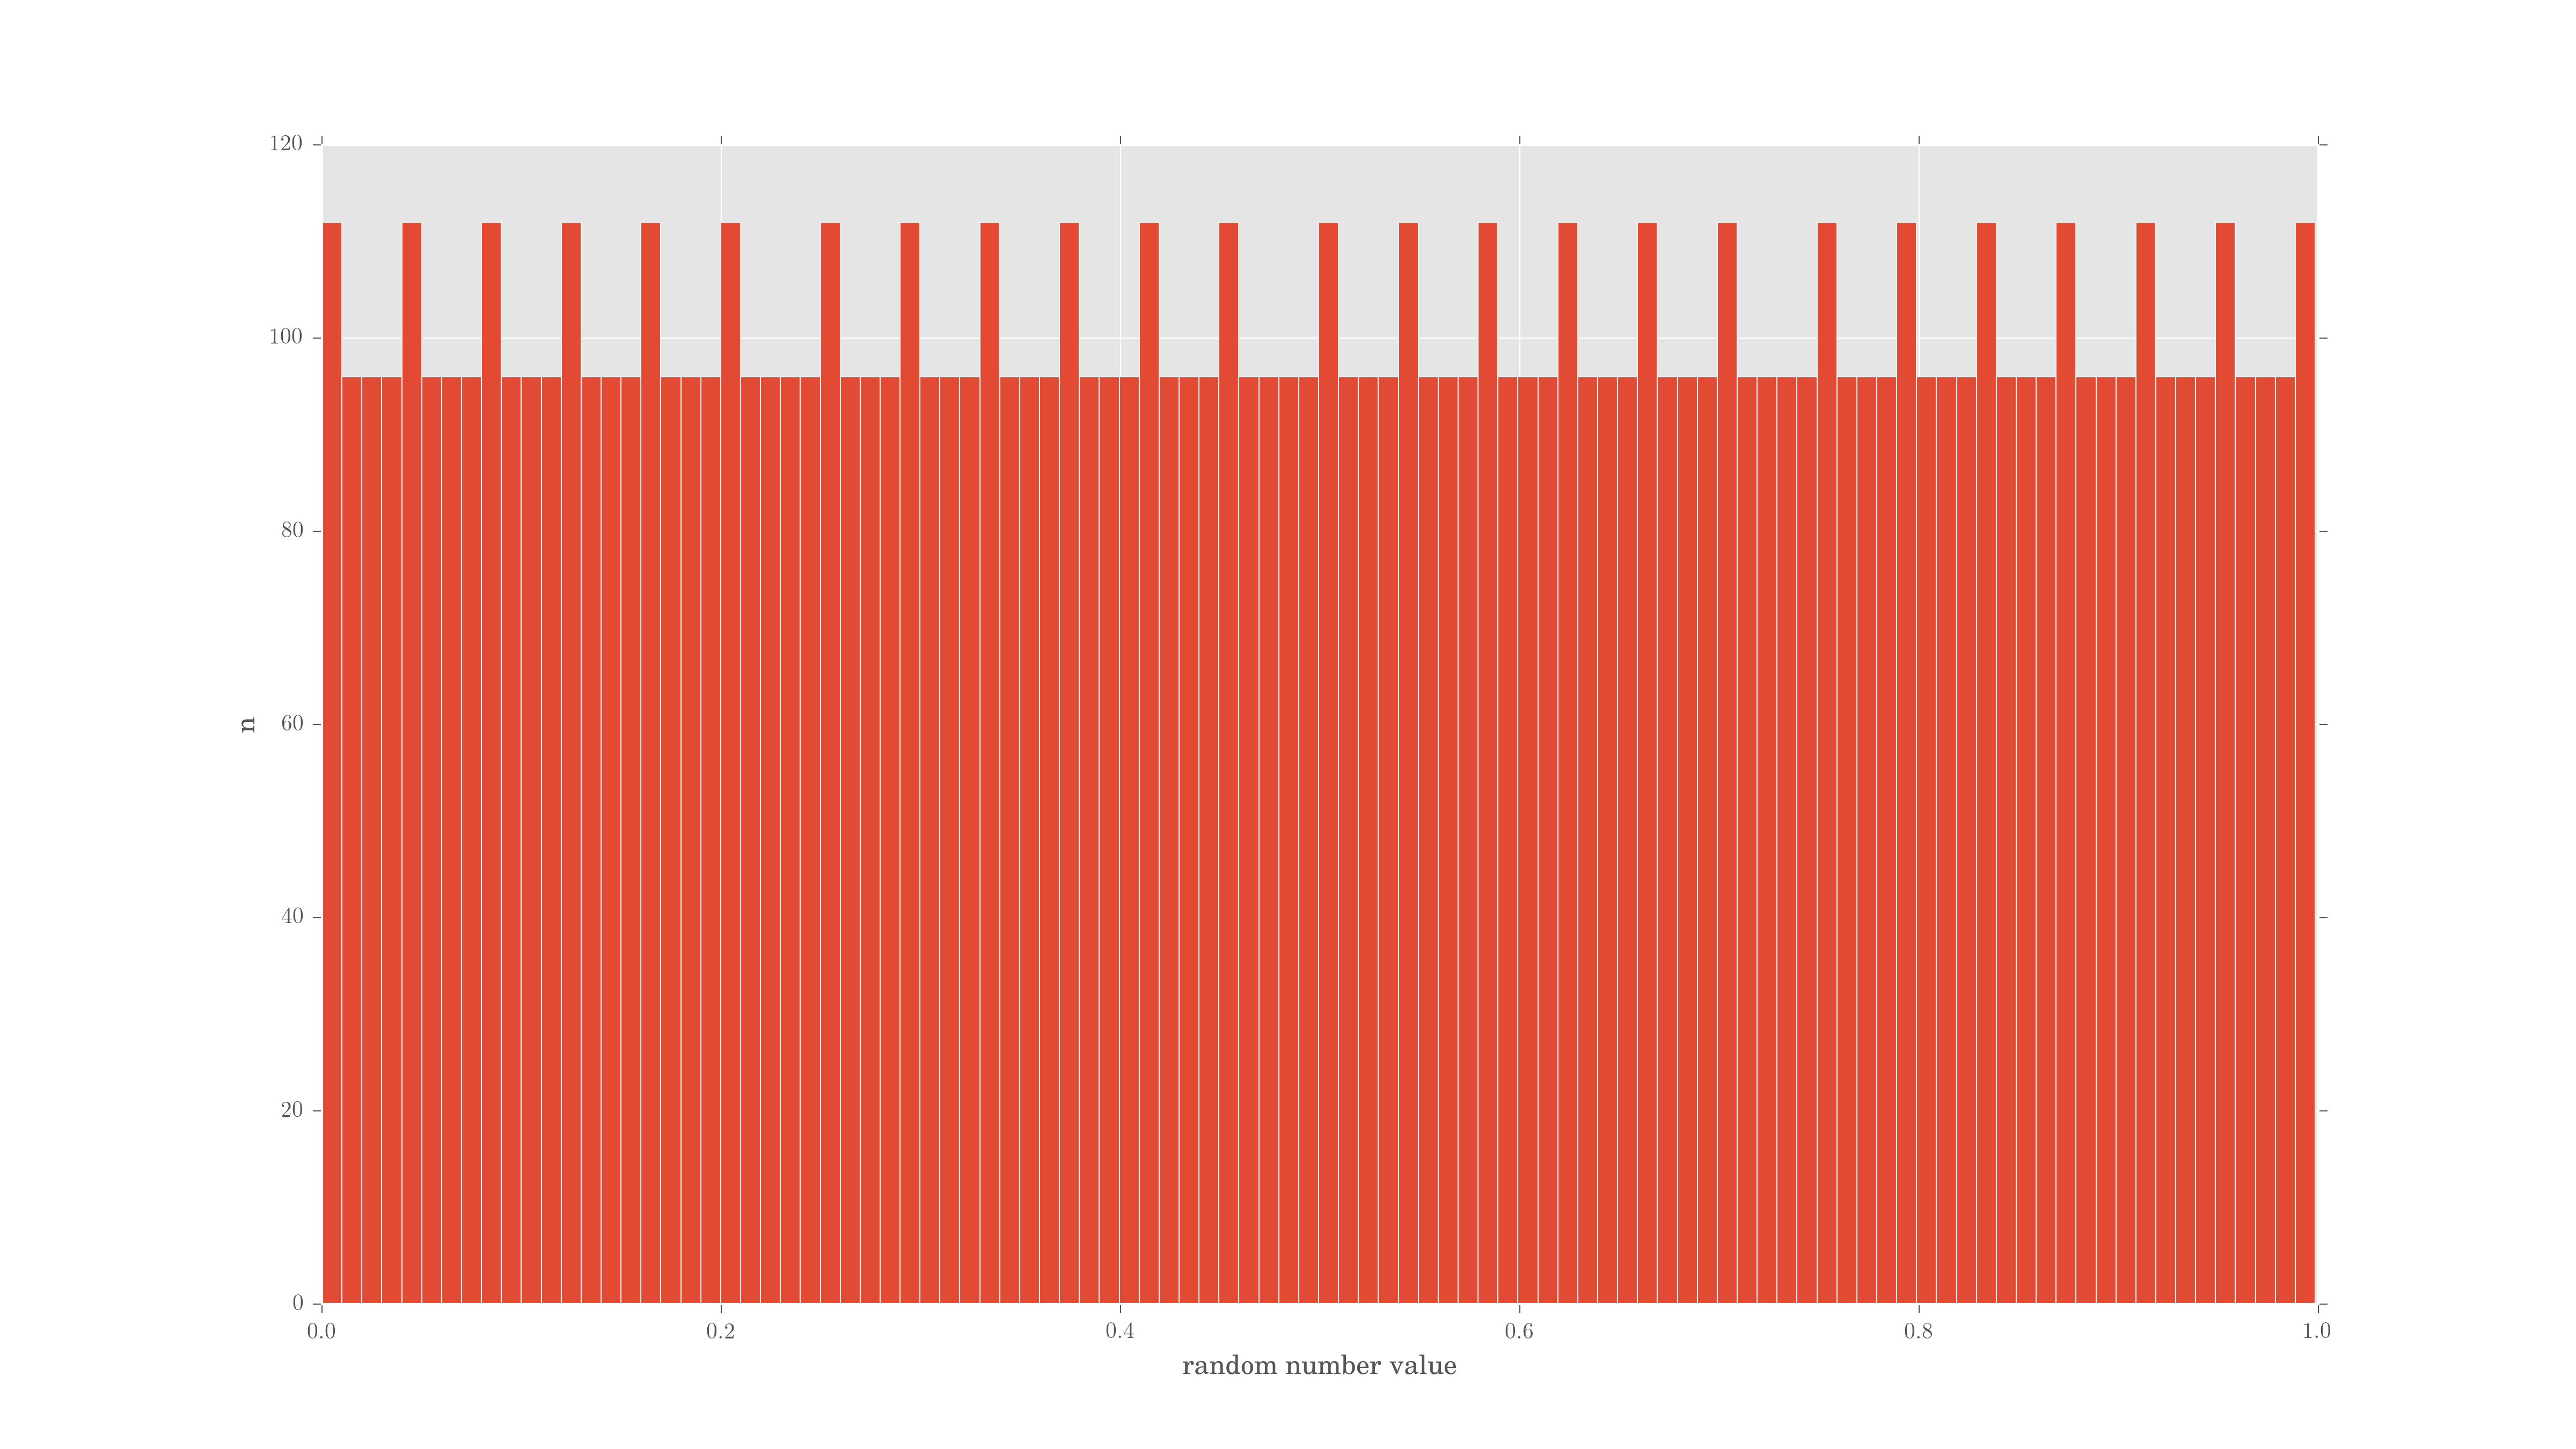
\includegraphics[width=\textwidth]{linear_kongruent_random_numbers.png}
\caption{$10000$ Zufallszahlen, erzeugt mit dem in Aufgabenteil a) programmierten Zufallszahlengenerator.}
\label{fig:2b}
\end{figure}
\item[c)] In den Histogrammen sind eindeutig Strukturen (Linien oder Ebenen) zu erkennen. Dies deutet darauf hin, dass Zahlen von den vorher generierten Zahlen abhängen und nicht komplett gleichverteilt sind.
\begin{figure}
\centering
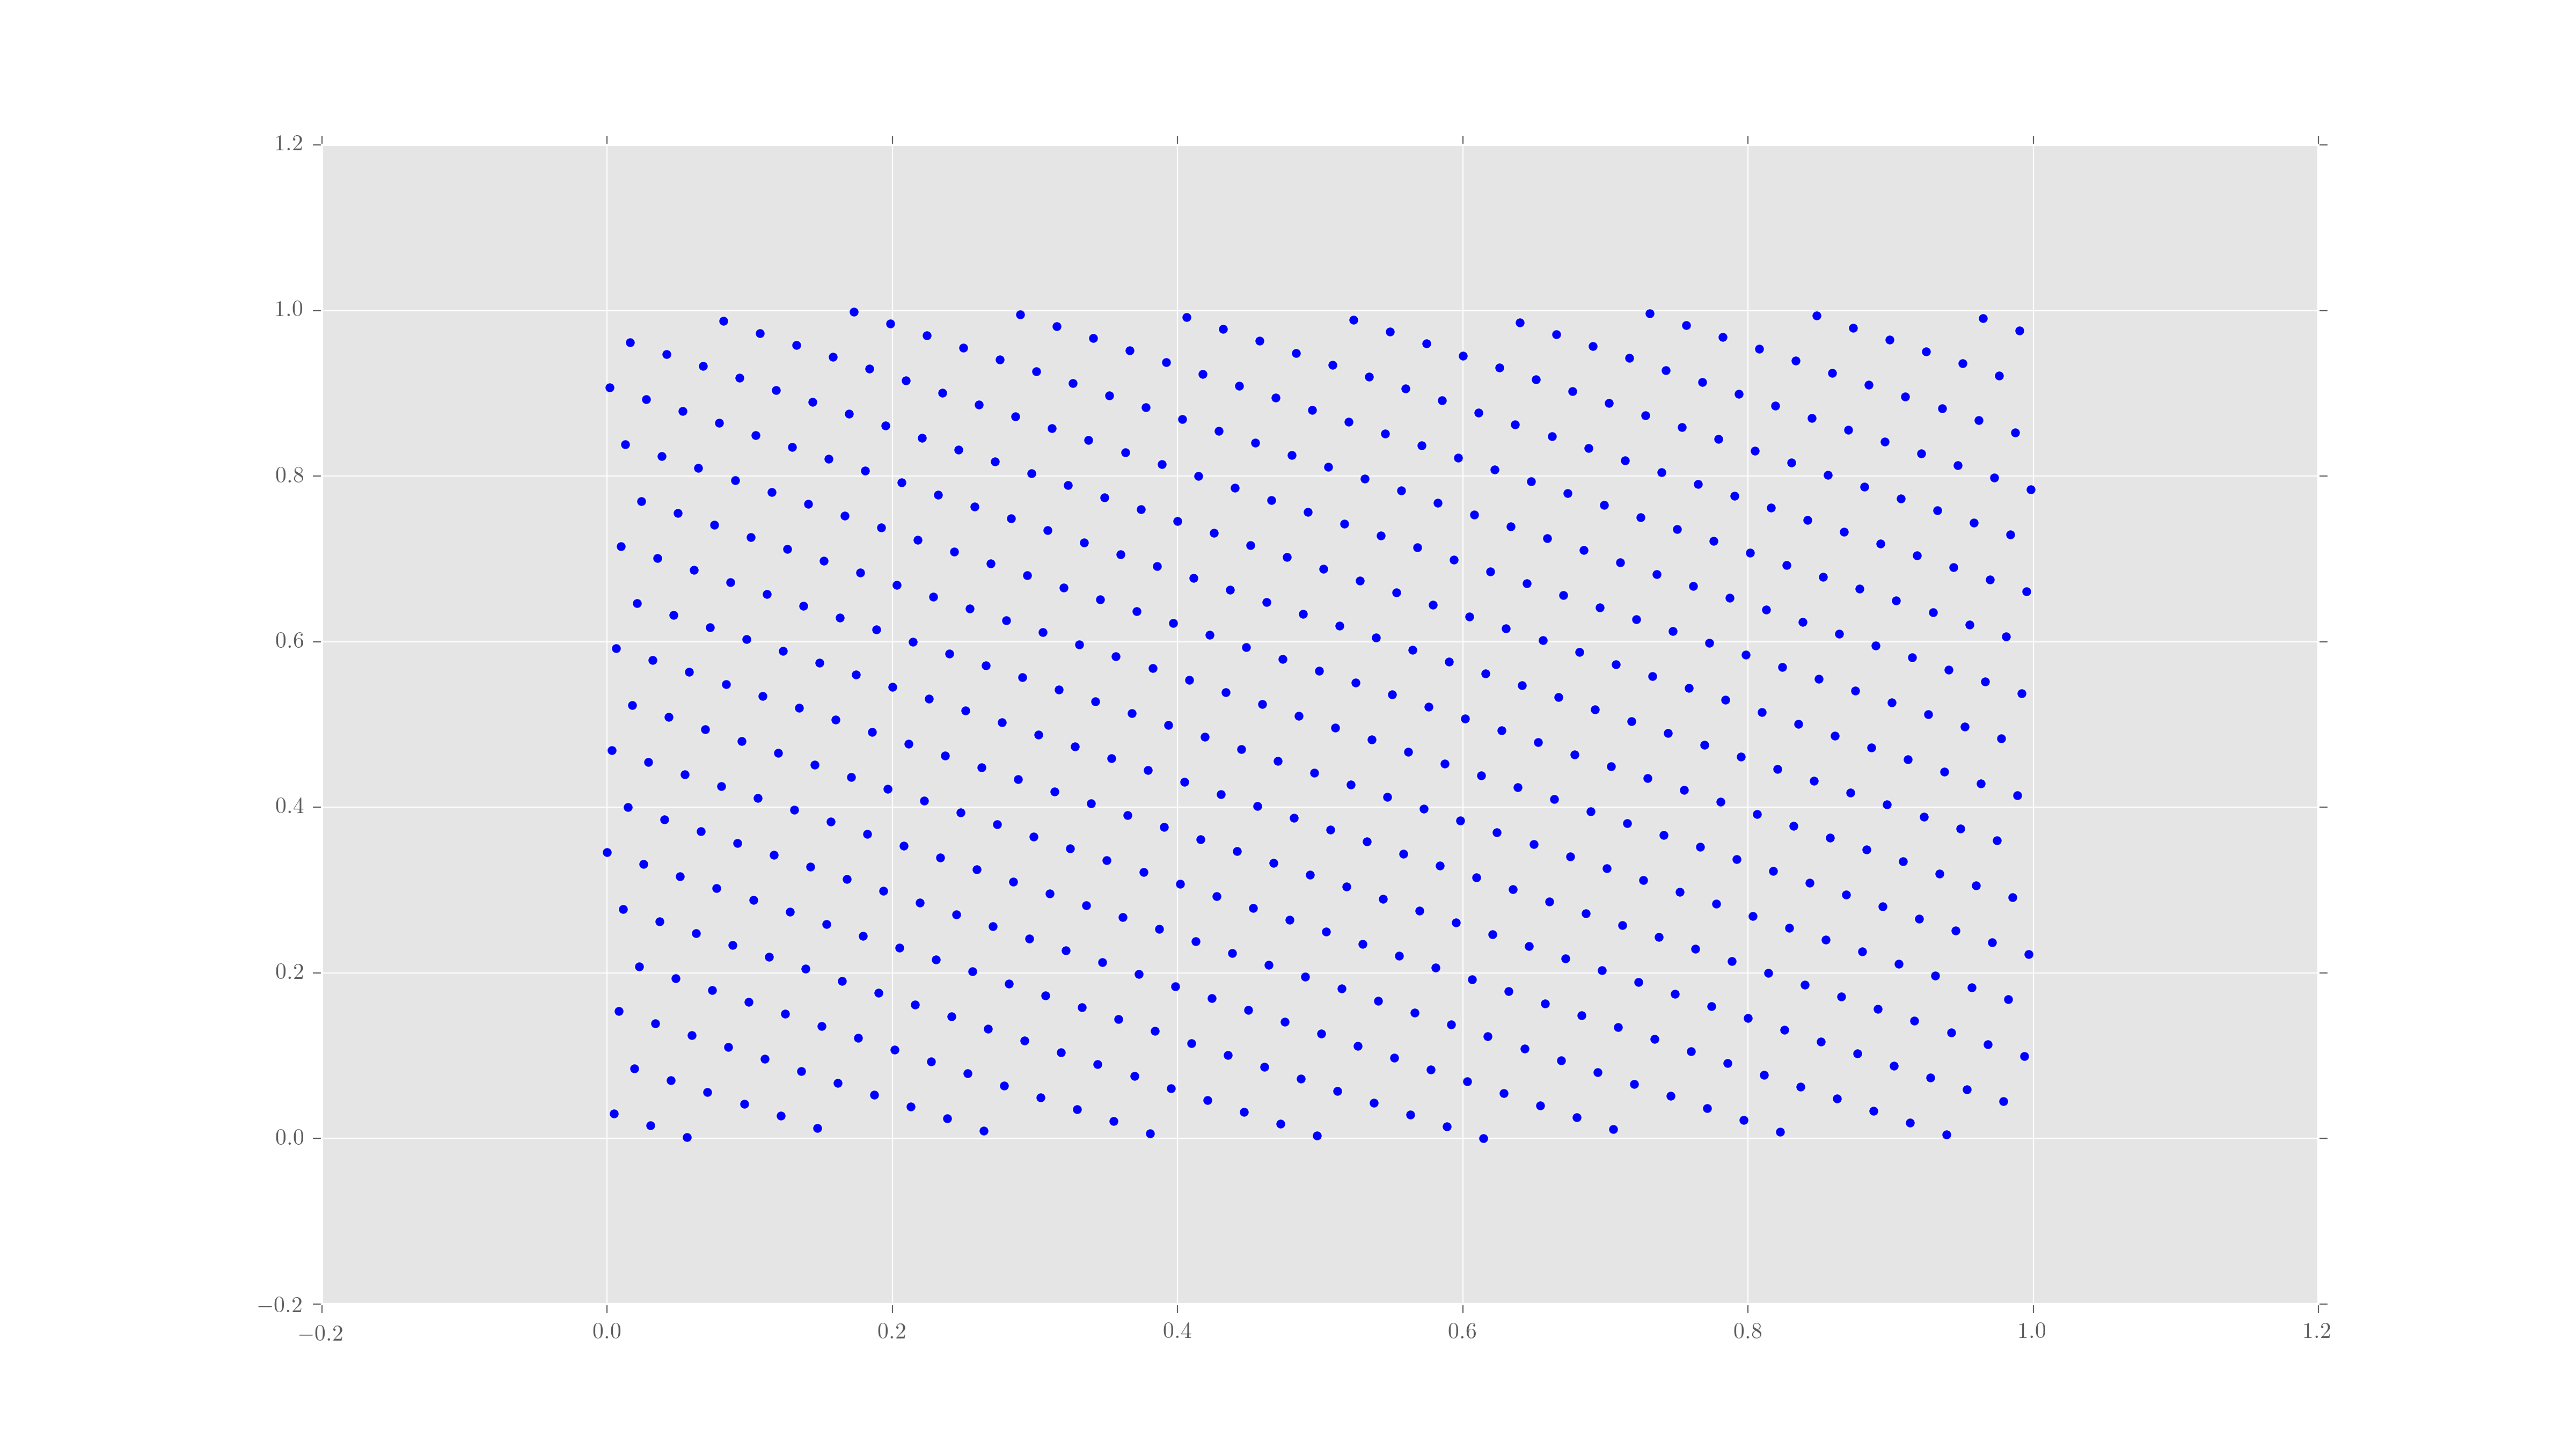
\includegraphics[width=\textwidth]{2dscatter.png}
\caption{Paare von Zufallszahlen, dargestellt als zweidimensionales Histogramm.}
\label{fig:2c1}
\end{figure}

\begin{figure}
\centering
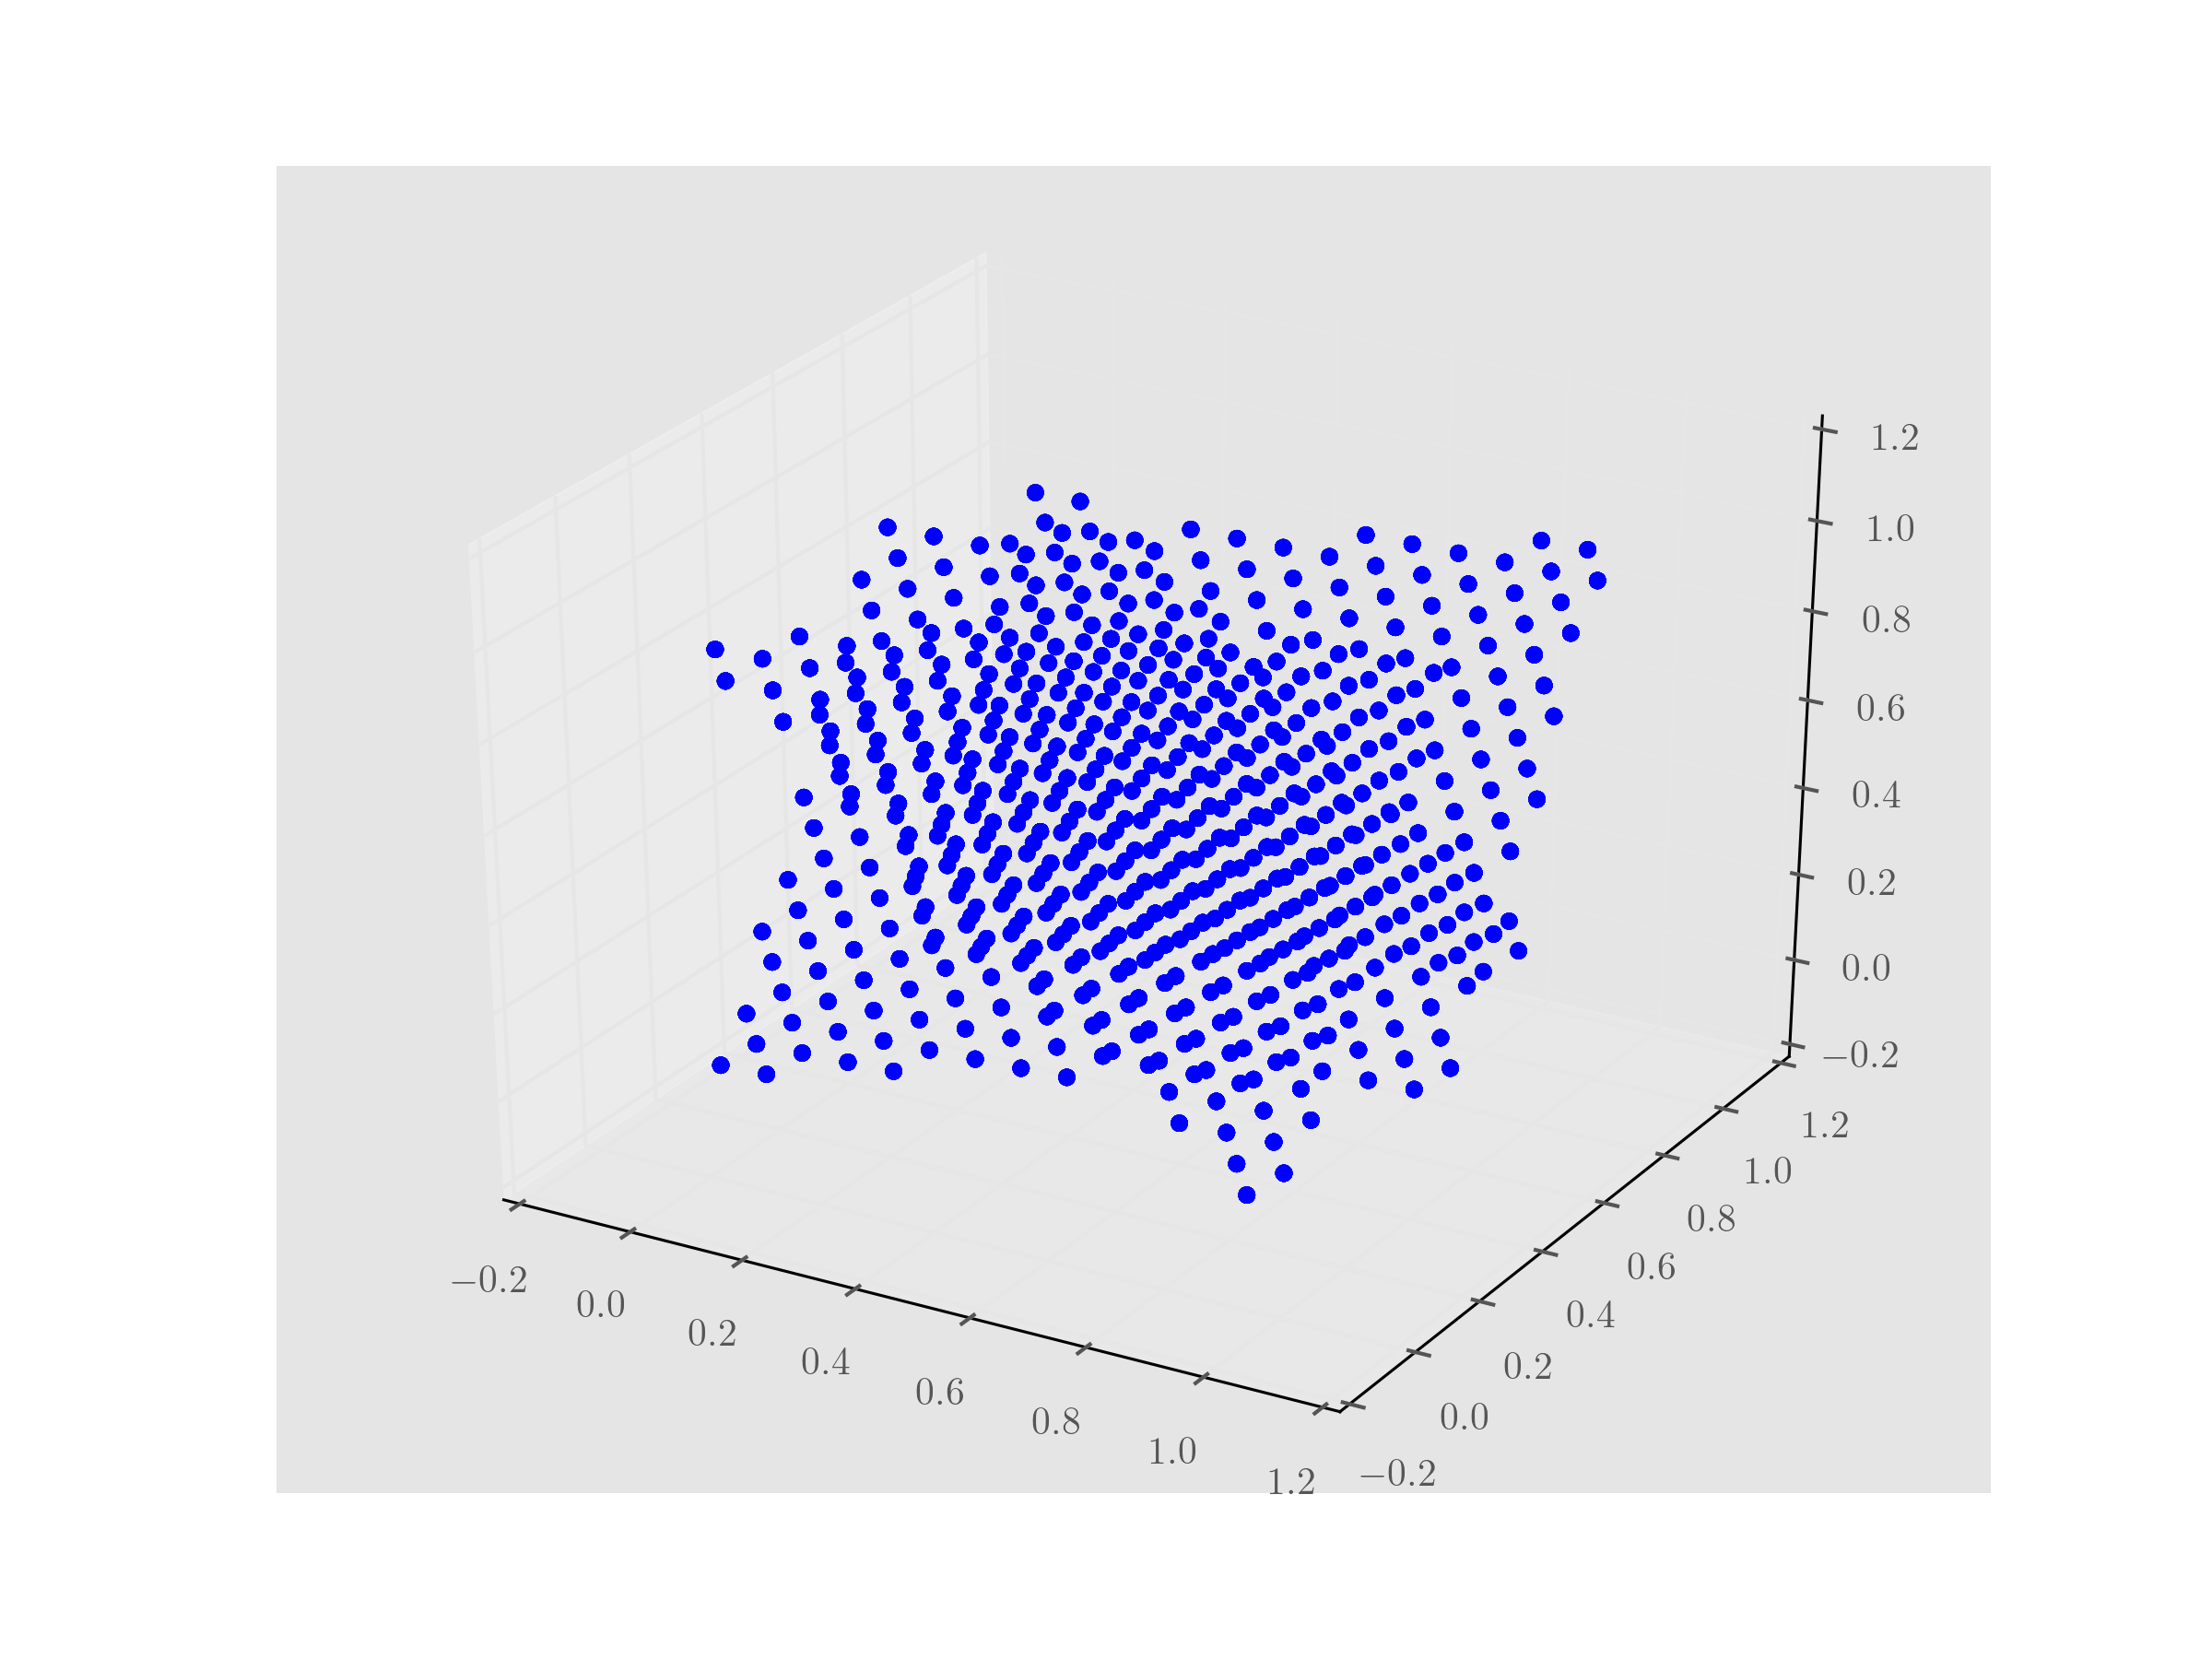
\includegraphics[width=\textwidth]{3dscatter.png}
\caption{Tripel von Zufallszahlen, dargestellt als dreidimensionales Histogramm.}
\label{fig:2c2}
\end{figure}
 

\begin{figure}
\centering
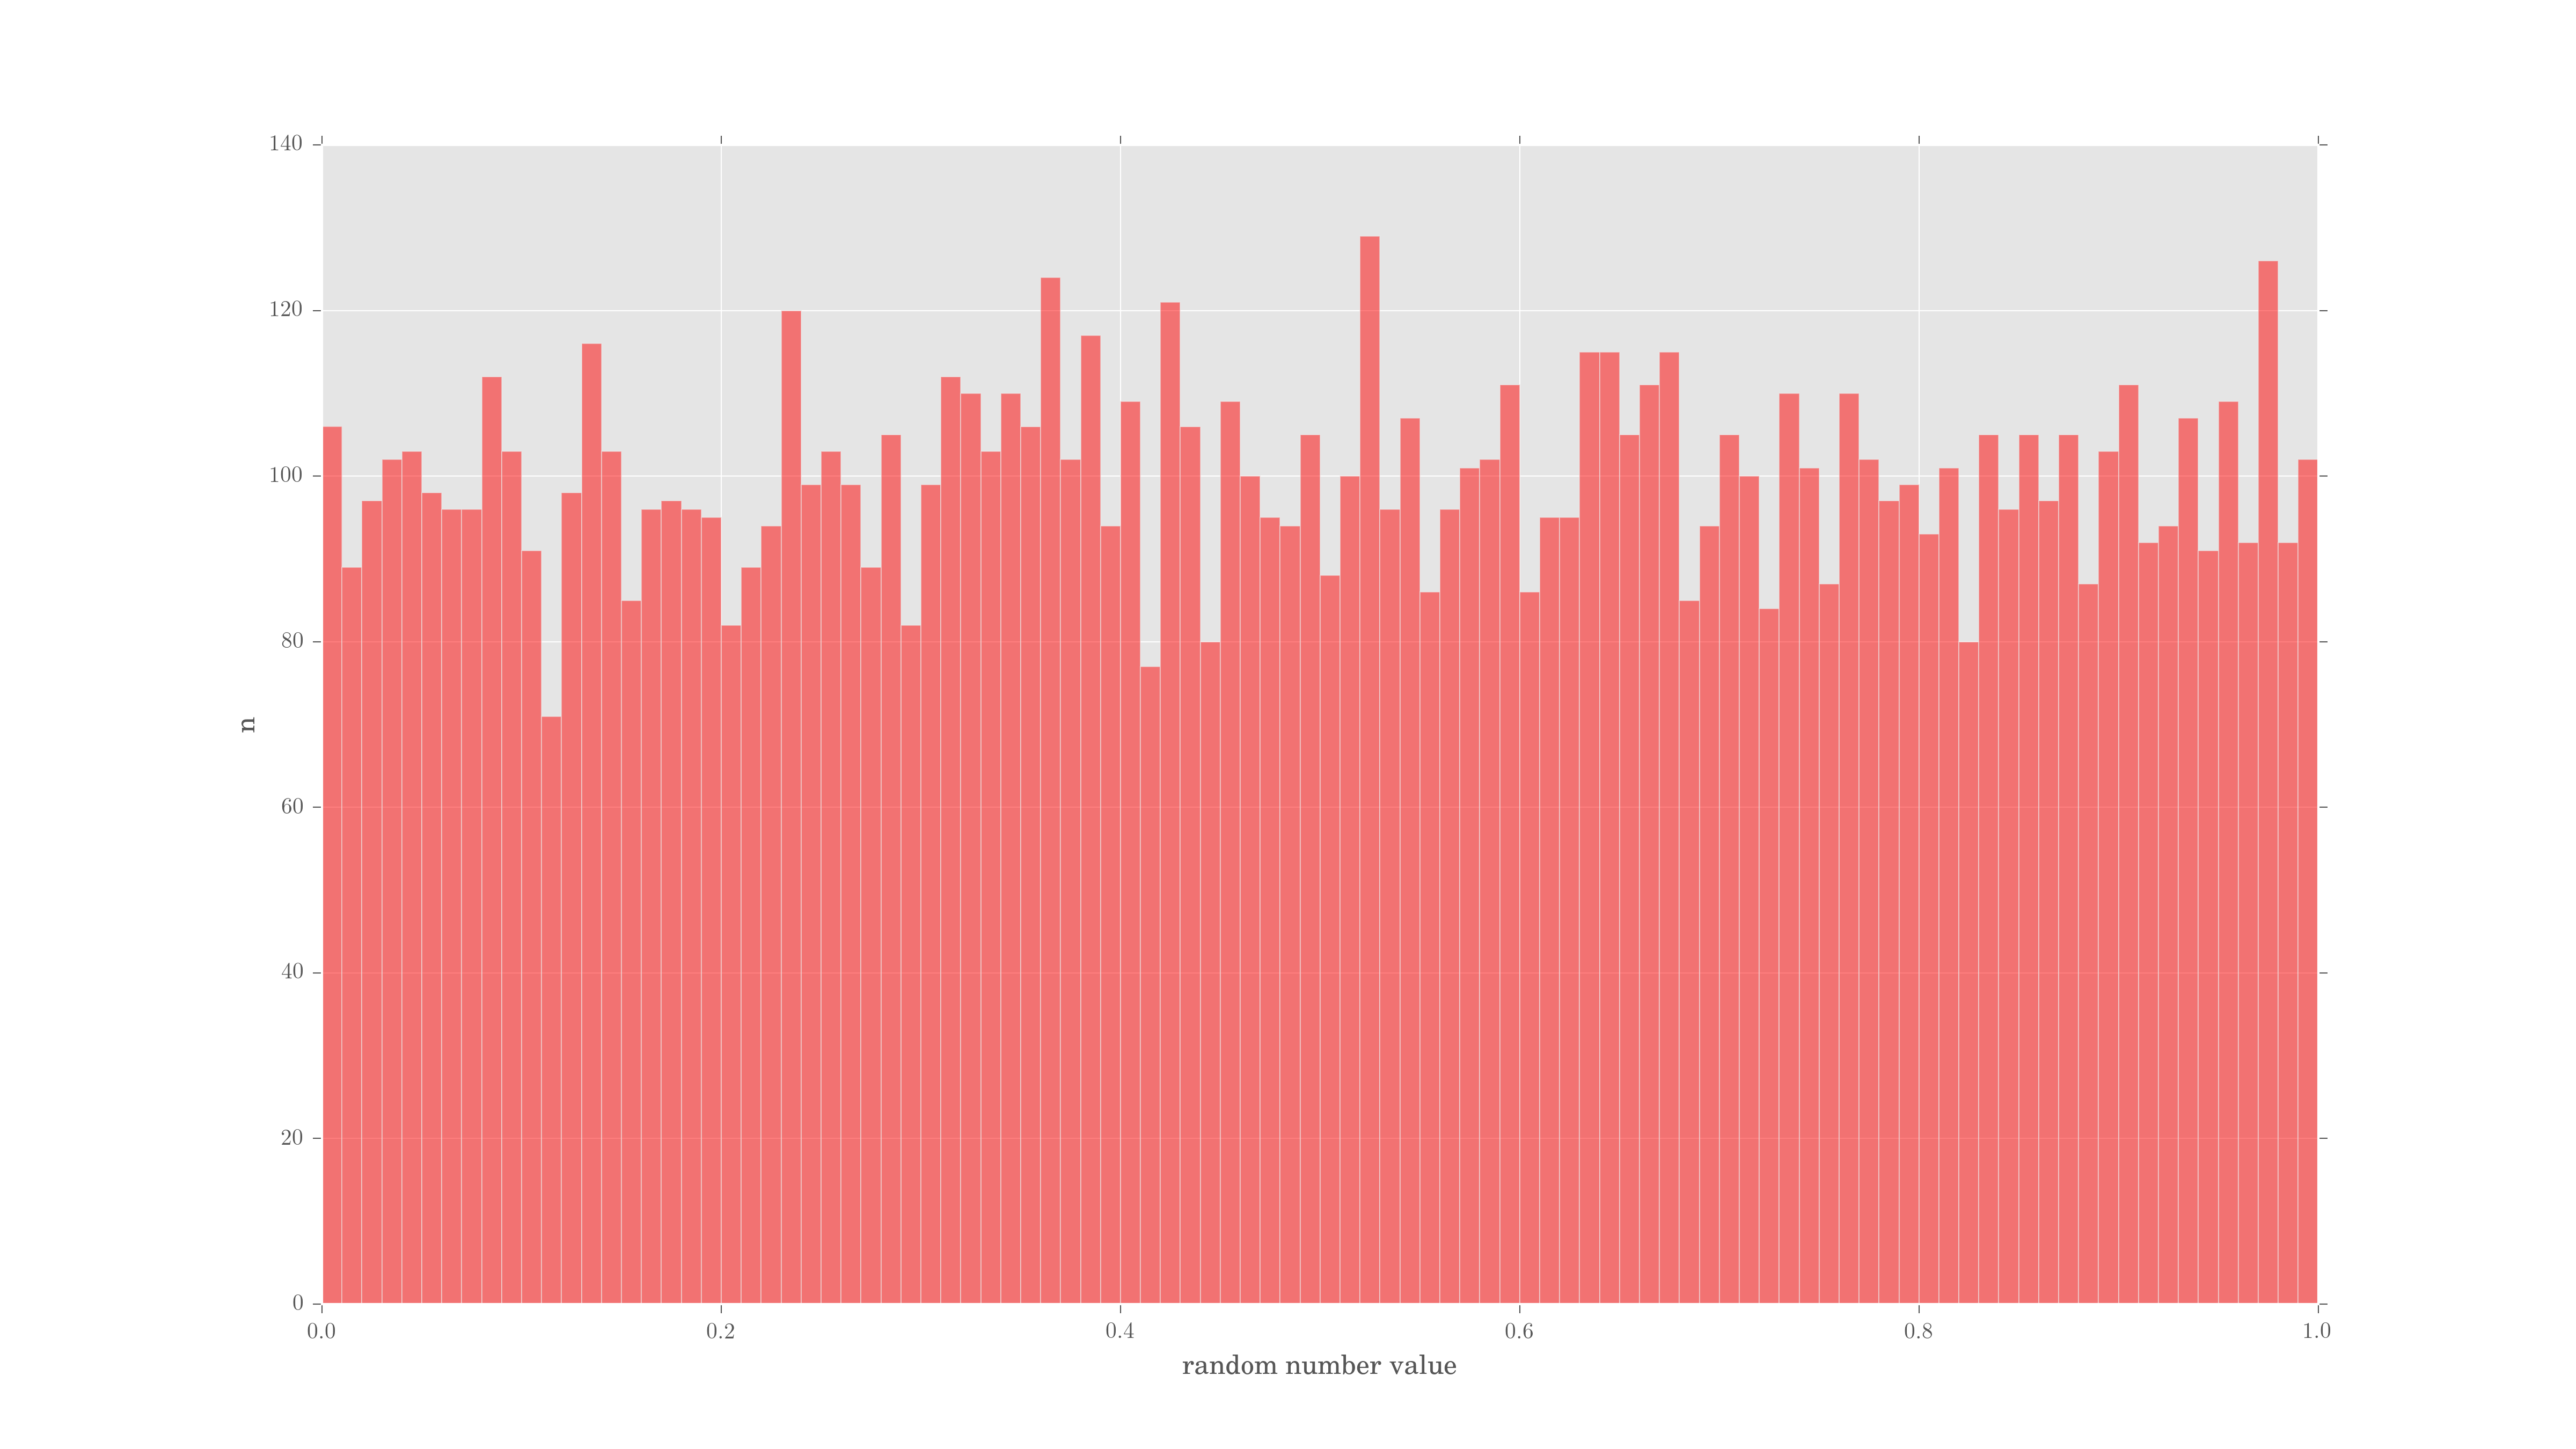
\includegraphics[width=\textwidth]{1dhist_root.png}
\caption{Mit ROOT erzeugte Zufallszahlen, dargestellt als Histogramm. Im Gegensatz zu dem vorherigen Histogramm lässt sich hier keine Struktur erkennen.}
\label{fig:2e1}
\end{figure}

\begin{figure}
\centering
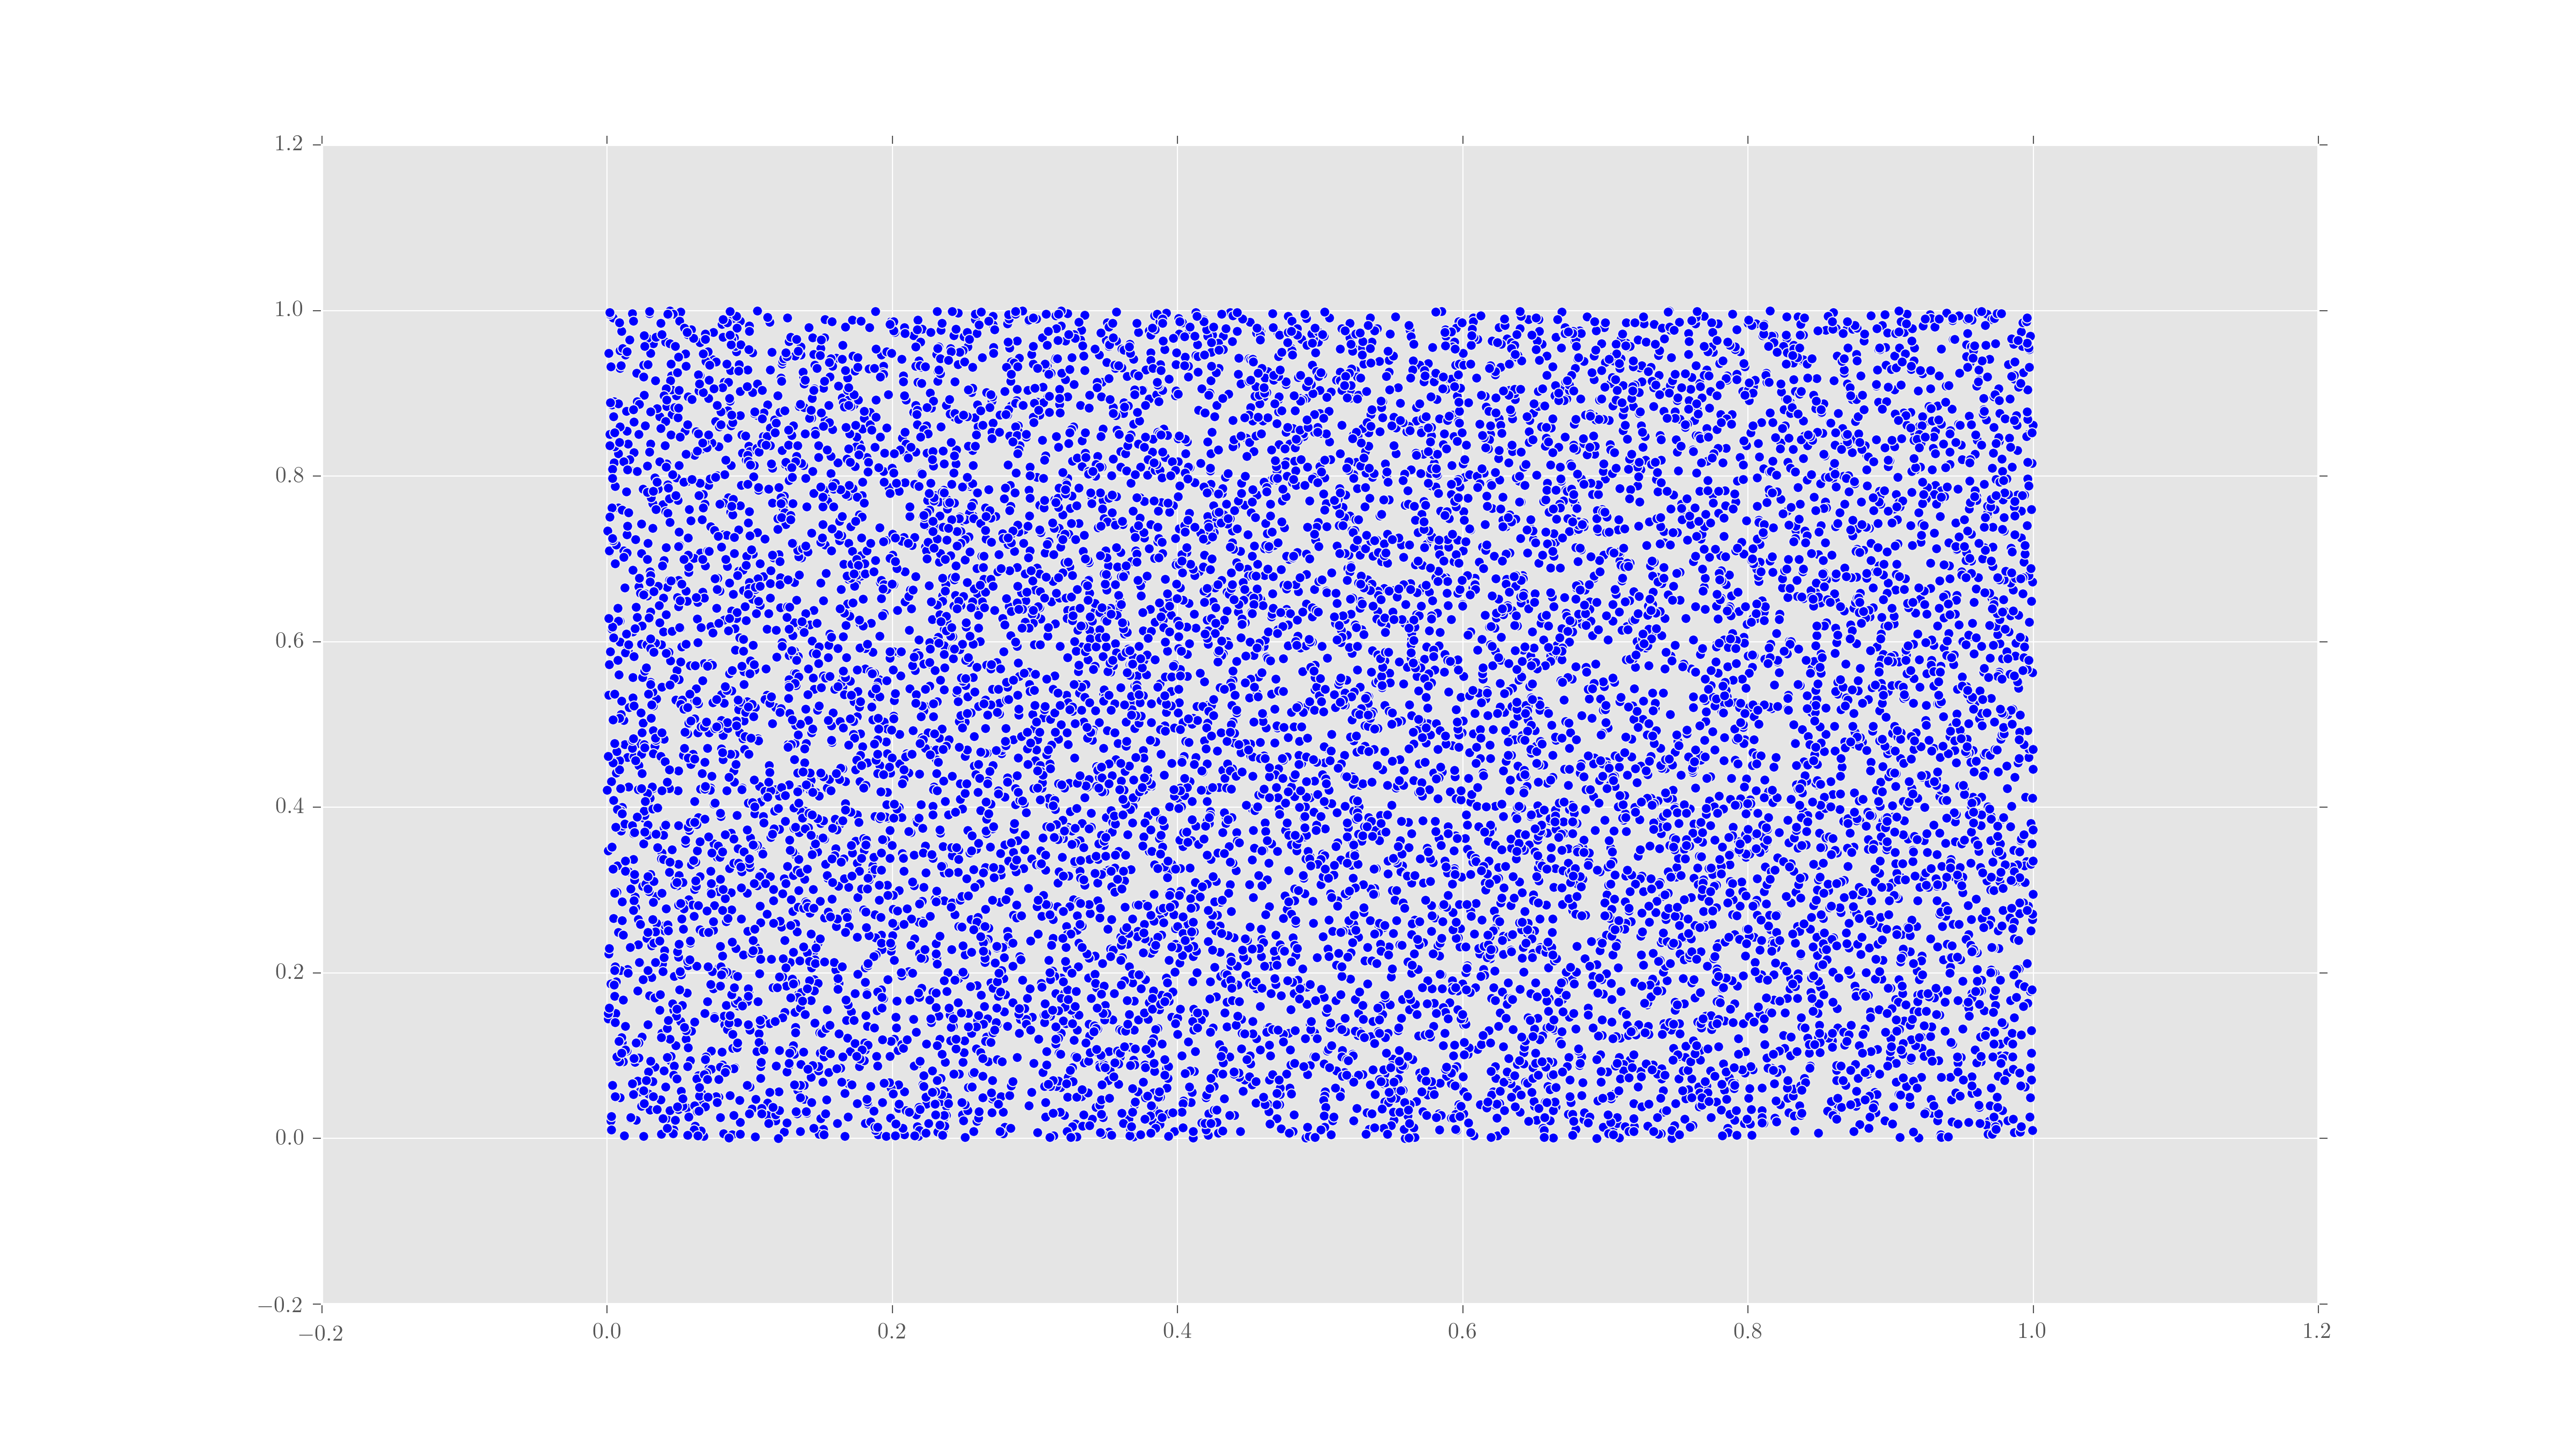
\includegraphics[width=\textwidth]{2dscatter_root.png}
\caption{Paare von Zufallszahlen, dargestellt als zweidimensionales Histogramm. Im Gegensatz zu dem vorherigen zweidimensionalen Histogramm lässt sich hier keine Struktur erkennen.}
\label{fig:2e1}
\end{figure}

\begin{figure}
\centering
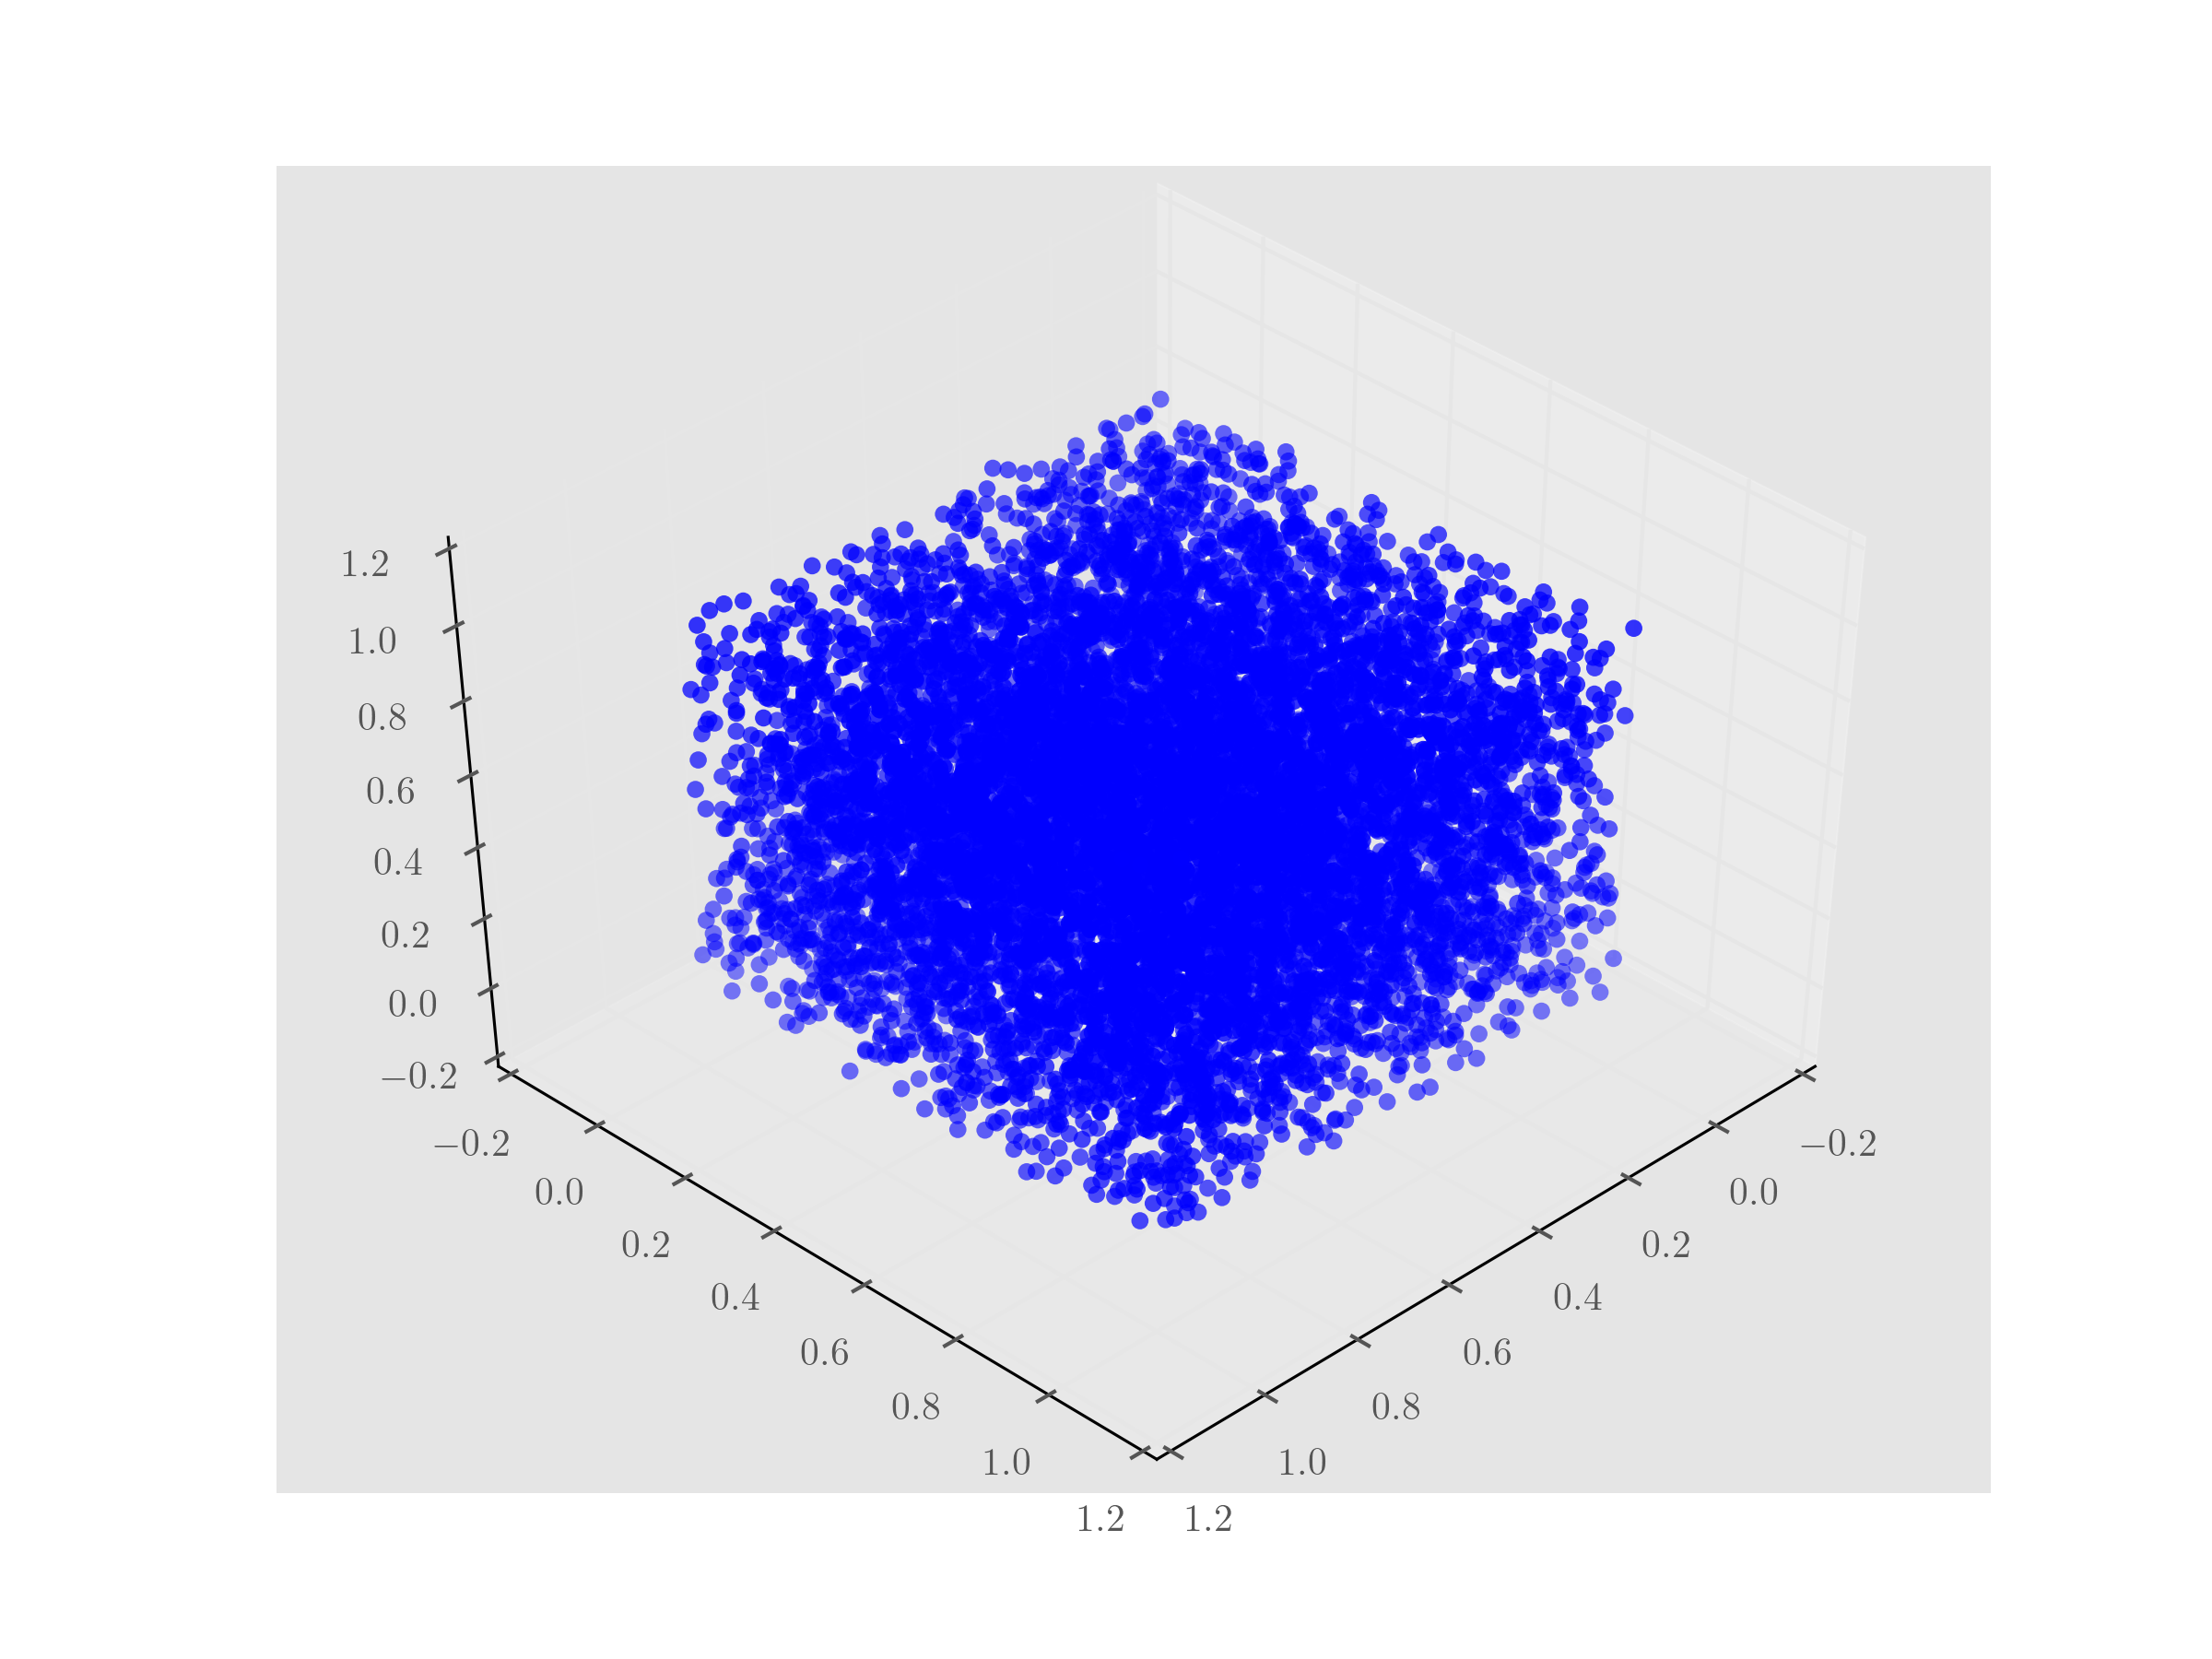
\includegraphics[width=\textwidth]{3dscatter_root.png}
\caption{Tripel von Zufallszahlen, dargestellt als dreidimensionales Histgramm.Im Gegensatz zu dem vorherigen dreidimensionalen Histogramm lassen sich hier keine Ebenen erkennen.}
\label{fig:2e2}
\end{figure}
\item[f)] Der mit den gegebenen Parametern Zufallsgenerator erzeugt nicht die Zahl $\num{0.5}$. Allerdings kann die Zahl $\num{0.5}$ erzeugt werden. Dafür wird der Algorithmus "invertiert" und es ergibt sich, dass, wenn $x_{ \text{seed} }=1144 + 10000k$ mit einer Ganzzahl $k$ , als Startwert gewählt wird die Zahl $\num{0.5}$ erzeugt wird.


\end{itemize}

\section*{Aufgabe 3: \emph{Zufallszahlengeneratoren}}
Hier werden die Transformierten Wahrscheinlichkeitsverteilungen aufgeführt.
\begin{itemize}
\item[a)]
\begin{align*}
f(x) = 1
\rightarrow x(r) =  (x_{max} - x_{min}) r + x_{min}
\end{align*}
\item[b)] 
\begin{align*}
f(t) = N e^{-t/\tau}
\rightarrow t(r) = -\tau \ln(1-r)
\end{align*}
\item[c)] 
\begin{align*}
f(x) = N x^{-n}
\rightarrow x(r) = ( r  (x_{max}^{1-n} - x_{min}^{1-n}) +x_{min}^{1-n})^{n-1}
\end{align*}
\item[d)]
\begin{align*}
f(t) = \frac{1}{\pi} \frac{1}{1+x^2}
\rightarrow x(r) = \tan\left(r-\frac{\pi}{2}\right)
\end{align*}
\end{itemize}

\section*{Aufgabe 4: \emph{Fehlerfortpflanzung}}
\begin{itemize}

\item[a)]
Mit den gegebenen Werten:
\begin{align*}
y &=a_0+a_1x \\
a_0&=a_1=1.0\pm0.2 \\
\rho& = \frac{\text{cov}(a_0,a_1)}{\sigma(a_0)\sigma(a_1)}=-0.8\\
\text{cov}(a_0,a_1)&=\rho \sigma(a_0)\sigma(a_1)=-0.8\cdot 0.2\cdot 0.2 = 0.032\\
\end{align*}
ergibt sich durch einsetzen für die Standardabweichung mit Berücksichtigung der Korrelation:
\begin{equation*}
\sigma_y = \sqrt{ 0.04 + 0.04x^2 - 0.064x }
\end{equation*}
und ohne Korrelation:
\begin{equation*}
\sigma_y = 0.2 \sqrt{1-x^2}
\end{equation*}
\item[b)] 
\begin{figure}
\centering
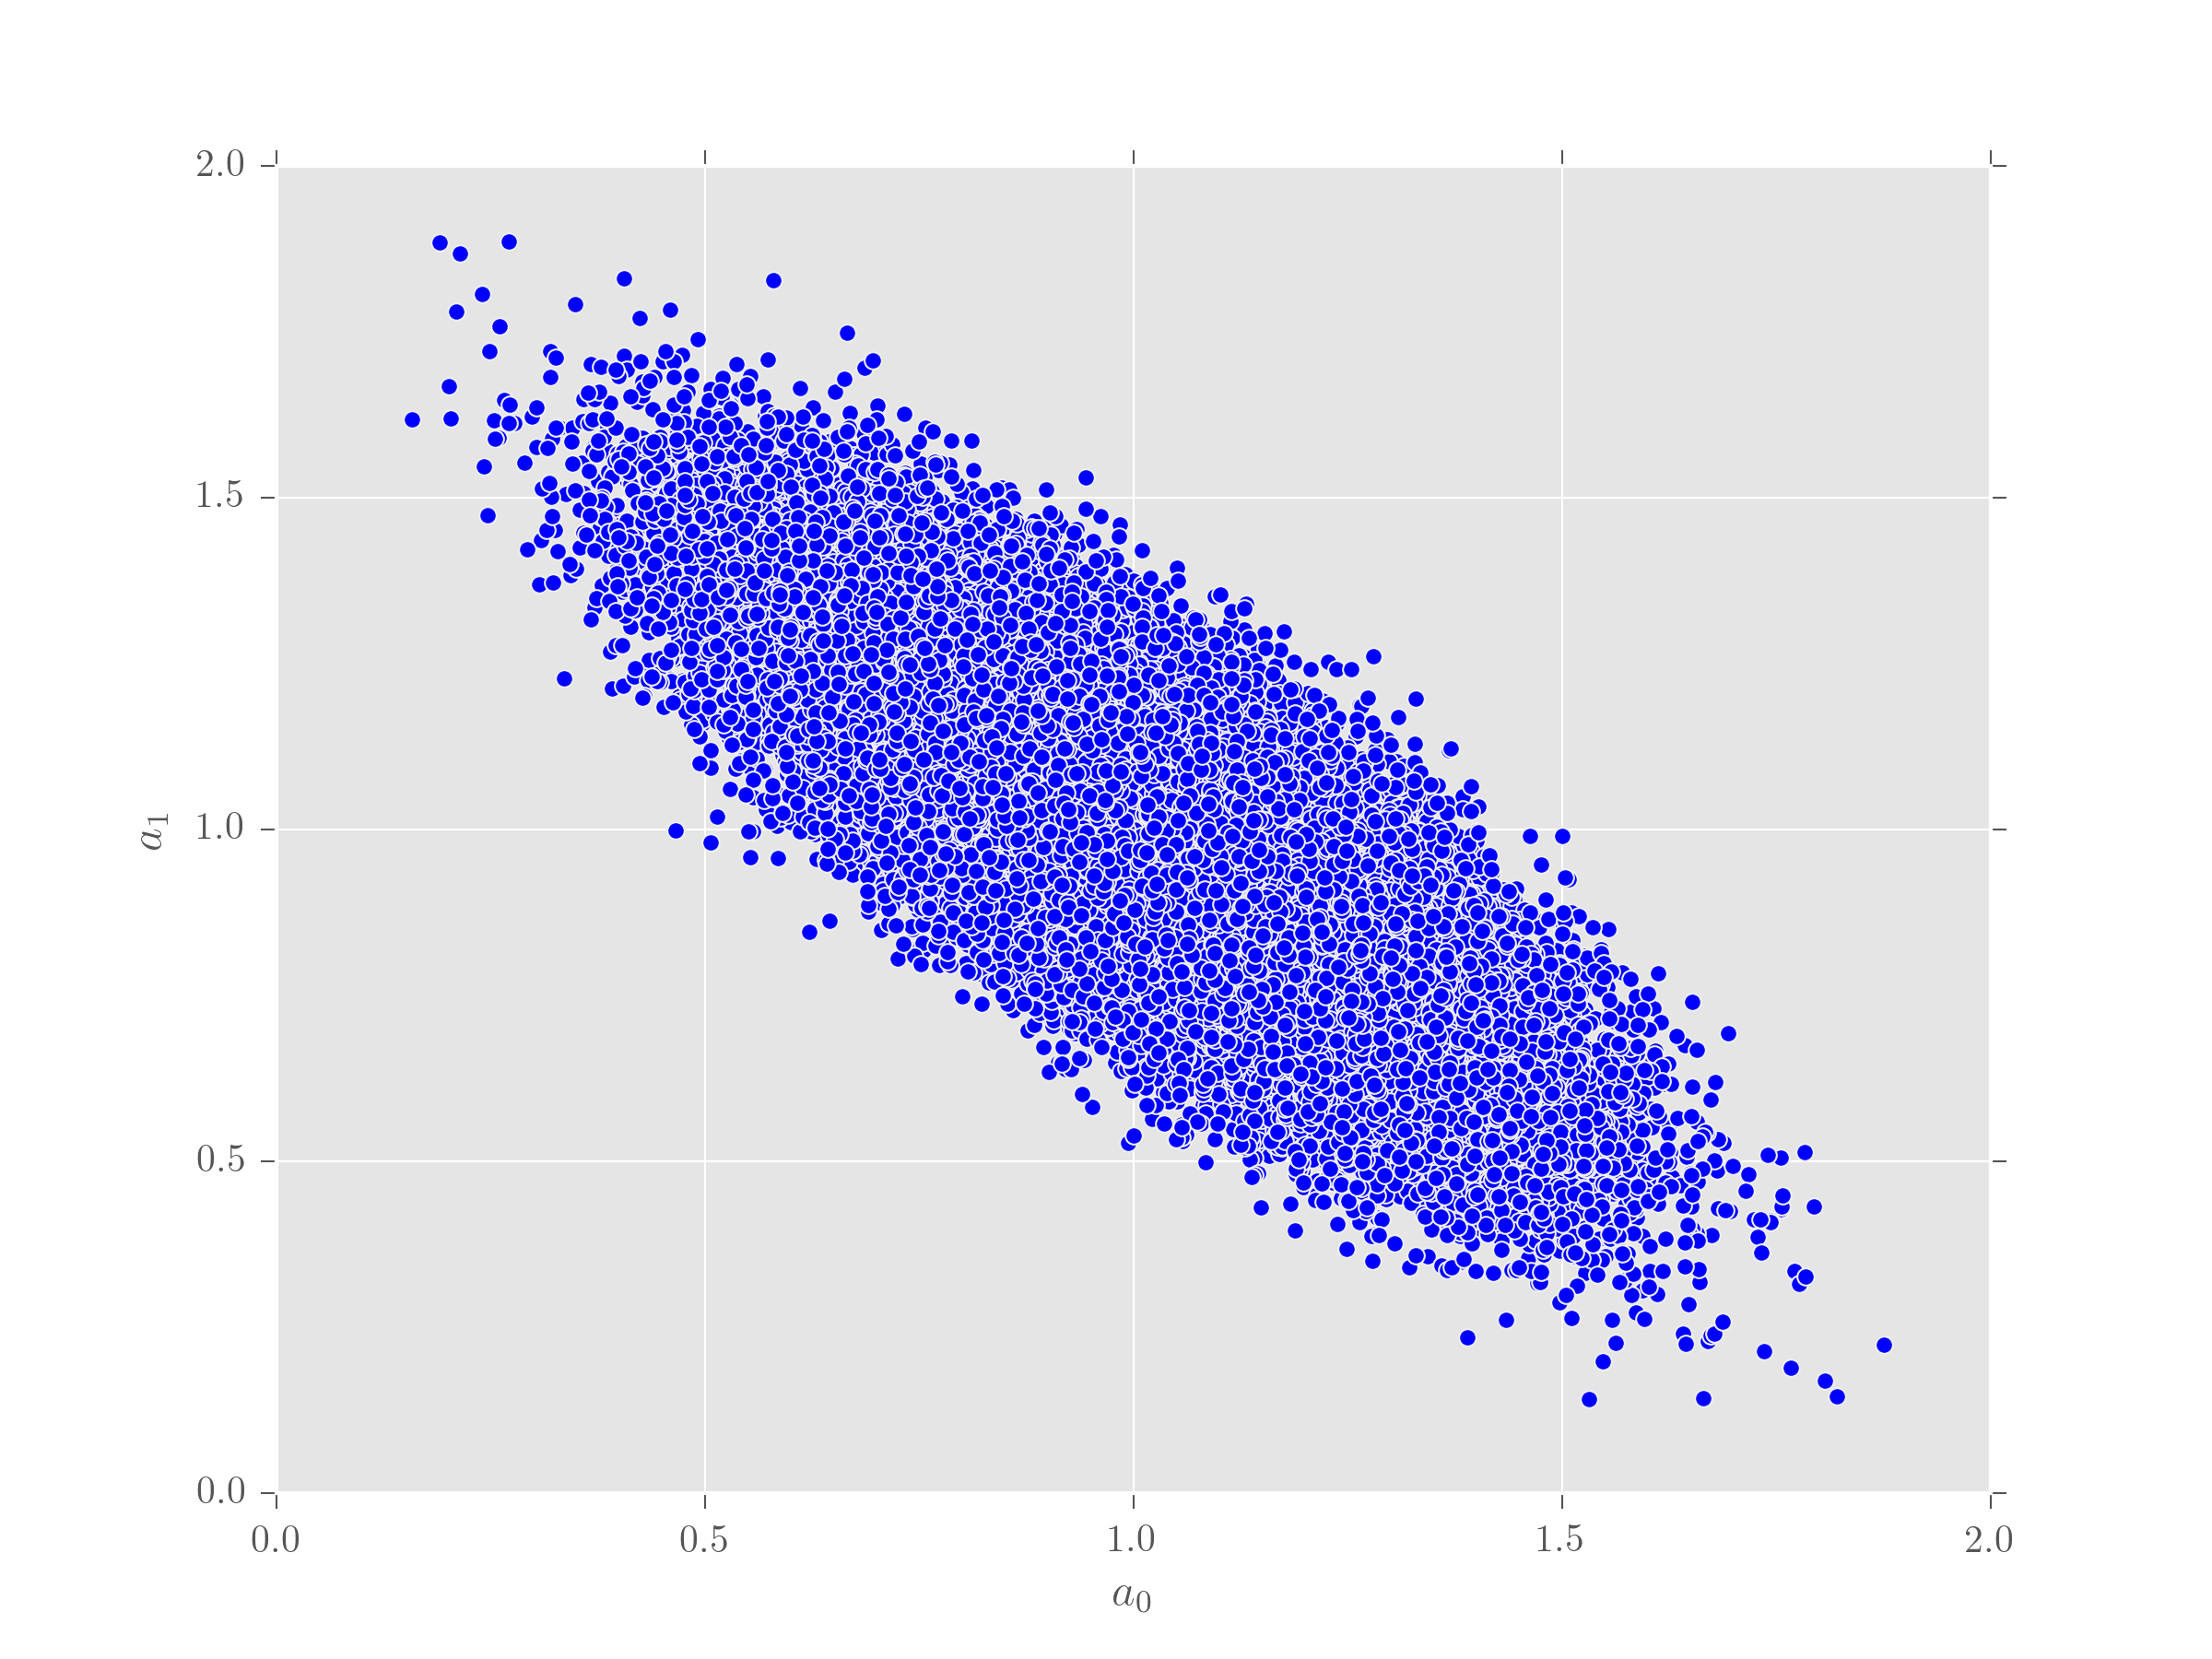
\includegraphics[width=\textwidth]{scatterplot_a0_a1.png}
\caption{Scatterplot für die Parameter $a_0$ und $a_1$ generiert durch normalverteilte Zufallszahlen mit angegebenem Mittelwert und Kovarianzmatrix.}
\label{fig:a0a1}
\end{figure}
\item[c)]
Die Vergleich von numerischer und analytischer Berechnung der Standardabweichung für $x = -3 , 0 , 3 $ liefert:
\begin{table}
\centering
\caption{Berechnung von $\sigma_y$}
\begin{tabular}{ccc}
$x$ & analytisch & numerisch \\
$-3$& $\num{0.7694}$ & $\num{0.7680}$ \\
$0$& $\num{0.2000}$ & $\num{0.1999}$ \\
$3$& $\num{0.4560}$ & $\num{0.4552}$ \\
\end{tabular}
\end{table}
Zur numerischen Berechnung wurden $\num{100000}$ Zufallszahlen verwendet.
\end{itemize}